%! Author = mariuszindel
%! Date = 24.01.21

\section{Accessibility}
\begin{center}
    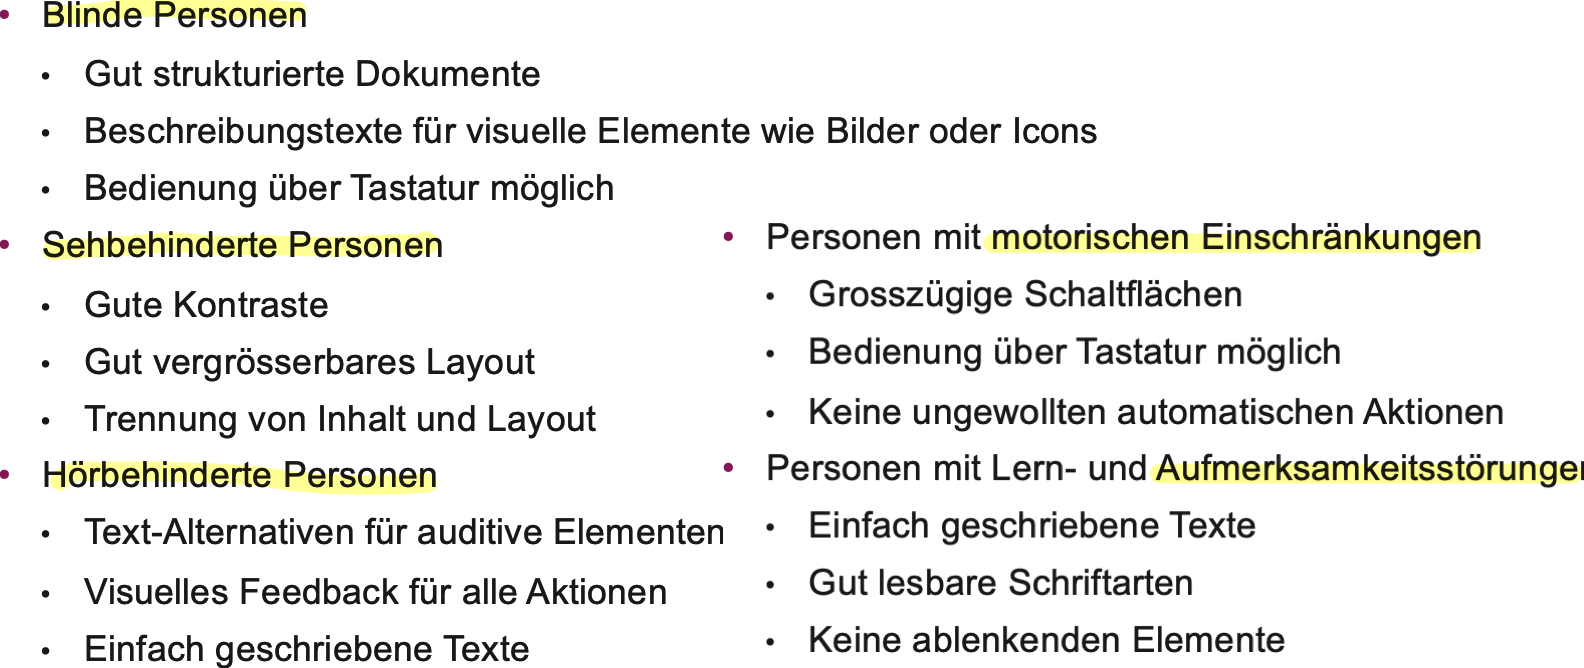
\includegraphics[scale=.2]{graphic/accessability/barrierefreien.png}
\end{center}
\vspace{-8pt}

\begin{itemize}
    \item keine Headings-level auslassen
    \item Semantic Elements richtig nutzen
    \item Skip-links am Anfang der Seite
    \item aria-hidden = nicht interessant für den Reader
    \item Bilder etc. mit angemessene textuelle Beschreibung(alt-Text)
    \item Keine Information ausschliesslich durch Farbe darstellen
    \item Vorder- / Hintergrund bei reduierter Farb- und Kontrastwahrnehmung in Standardansicht deutlich unterscheidbar
    \item Skalierung der Schrift über Funktionen des Browers möglich (em/rem und \% statt px)
    \item Jede Funktion ist über Verwendung der Tastatur in schlüssigen Reihenfolg erreichbar
    \item Tabelle: sprechende Column- \& Row-headers 
\end{itemize}


\subsubsection{Star-Rating}
\begin{itemize}
    \item visuallyhidden für Sterne verwenden
    \item Elimination der dynamischen DOM-Abfragen
\end{itemize}

%\subsection{Sehschwäche}

%\subsubsection{Farbenblindheit}
% Techniken aufzählen wie Web-UI sinnvoll für Farbenblindeheit optimiert werden können.
%Testen:
%\begin{lstlisting}
%:root {
%filter: grayscale(100%) !important; }
%\end{lstlisting}
%
%\subsubsection{Kontrast}
% erklären warum Optimierung für Farbblindheit und Optimierung des Farbkontrasts von Web-UI Elementen nicht das Gleiche ist .


%\subsection{Zoombarkeit}
% erklären warum Zoombarkeit von Web-Uis wichtig ist, und welche Praktiken vermieden werden sollten.


%\subsection{Animationen}
% erklären warum Animationen in Web-UI abgestellt werden können sollen.


%\subsection{Auszeichnung von Medien}


%\subsection{Screen-Reader}





% Überprüfungsvorschläge des Chrome Accessibility Checks in einem Kontext in Handlungsempfehlungen übersetzen.
% die Accessibility von Formularen und Tabellen beurteilen und optimieren.





\columnbreak